
    In this section we outline the estimated impact of MW changes on rent and house prices. We start by showing the results of our event-study specification with one event per zipcode. As discussed extensively in section \autoref{sec:empirical_strategy}, this model suffers from underidentification issues. We show several ways in which we address those. Later, we present results for the first difference specification, which we deem more reliable. Finally, we discuss the magnitude of the estimates.


\subsection{Event-study specification}\label{subsec:results/event-study}

    We being discussing the results by presenting our estimation of the last event specification using median rents per square foot as our main dependent variable. In particular, we focus on the median rent per square foot for single family houses and condos (SFCC) as this is the most populated time series in the Zillow rent data. We show the robustness of our results by using alternative rent variables in Appendix Figure \ref{appfig:event_study_change_depvar}.
    As described in the data section, we also fix the composition of the panel by using zipcodes with valid rents data as of June 2015.\footnote{It is worth emphasizing that the panel is still not balanced. The reason is that Zillow started to provide data on these zipcodes at different points in the period 2010-2015.} The concern we address here is that a changing composition of the sample may bias the results.
    
    Figure \ref{fig:event_study_main} shows different specifications of the ``last event'' event-study discussed in section \ref{sec:empirical_strategy}. The first row shows results of the basic two-way fixed effect model in equation \eqref{eq:last-event-study}, using only zipcodes that experience some MW change in the period of interest. Panel (a) controls only for unused MW events, whereas panel (b) adds county-specific linear and quadratic trends. Although this latter panel suggests a mild but non-significant increase in rents after the last MW change, overall these plots suggest no effects on rent. However, we do not trust on these results for several reasons. First of all, \textcite{BorusyakJaravel2017} show that the dynamic coefficients in this model are under-identified. Secondly, by dropping untreated units we use a rather small sample, which means that confidence intervals are relatively large. The remaining panels attempt to address these issues.
    
    While using the same sample of untreated units as (a) and (b), panels (c) and (d) tackle the underidentification problem by replacing zipcode with county fixed effects (equation \eqref{eq:last-event-study-countyFE}). The results are in fact very similar to the basic TWFE, showing a mild increase in the dynamic effects once county-specific trends are included. 
    
    Finally, the third row shows the results of fitting equation \eqref{eq:last-event-study-control}. This specifications keep zipcodes fixed effects, but also add add geographical units that were never treated to the estimating sample. Panel (e) shows a strongly significant effect. Monthly median rent per square foot is around \$0.03 higher 6 months after the MW with respect to the month before the implementation (s.e. 0.0081). This implies that a house of 1,000 square feet would increase its rent around \$30.
    % Full regression output: https://github.com/diegogentilepassaro/min_wage_rent/blob/9403cb9f01217ed02c9d5bf8ea3138430227c0f7/analysis/event_study/output/make.log#L762-L814
    Panel (f) aims at controlling for unobserved trends in rents in local markets that may confound the effect, adding a county-specific linear and quadratic trend. The resulting dynamic effects seem to be slightly lower, and confidence intervals sometimes cross 0. 
    
    \begin{figure}[h!] \centering
        \caption{Dynamic effects around selected minimum wage events: rents}
        \label{fig:event_study_main}
        \begin{subfigure}{0.5\textwidth} \centering
            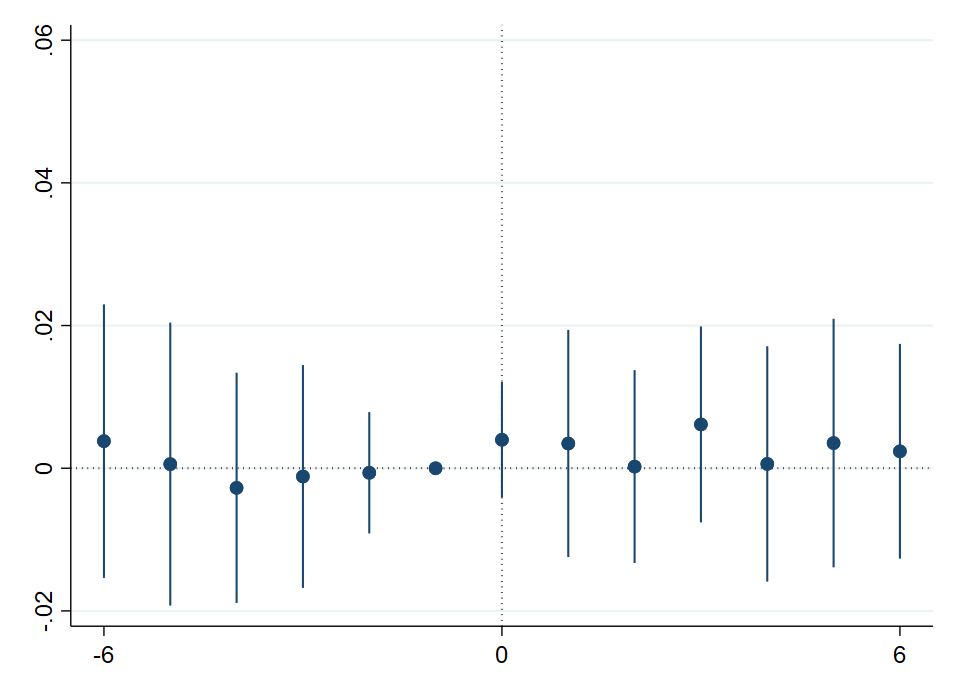
\includegraphics[width=0.95\linewidth]{analysis/event_study_exploration/output/last_rentpsqft_sfcc_zfe_w6.png}
            \caption{Basic TWFE with treated units only} \label{fig:event_study_treated}
        \end{subfigure}%
        \begin{subfigure}{0.5\textwidth} \centering
            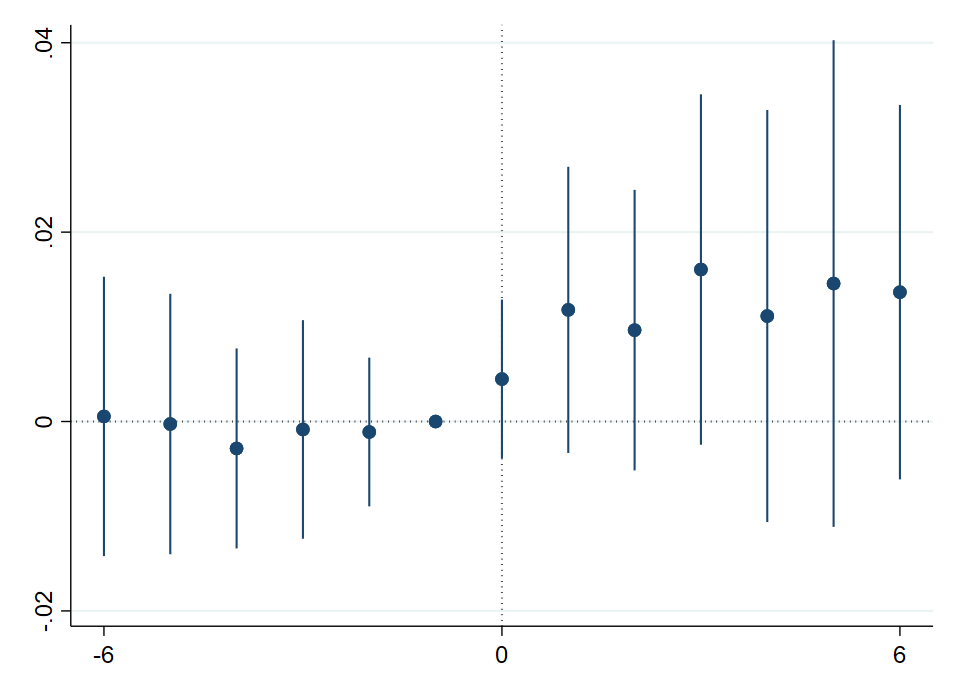
\includegraphics[width=0.95\linewidth]{analysis/event_study_exploration/output/last_rentpsqft_sfcc_zfe_w6_county-trend.png}
            \caption{Basic TWFE and county-specific trend} \label{fig:event_study_treated_county-trends}
        \end{subfigure}\\
        \begin{subfigure}{0.5\textwidth} \centering
            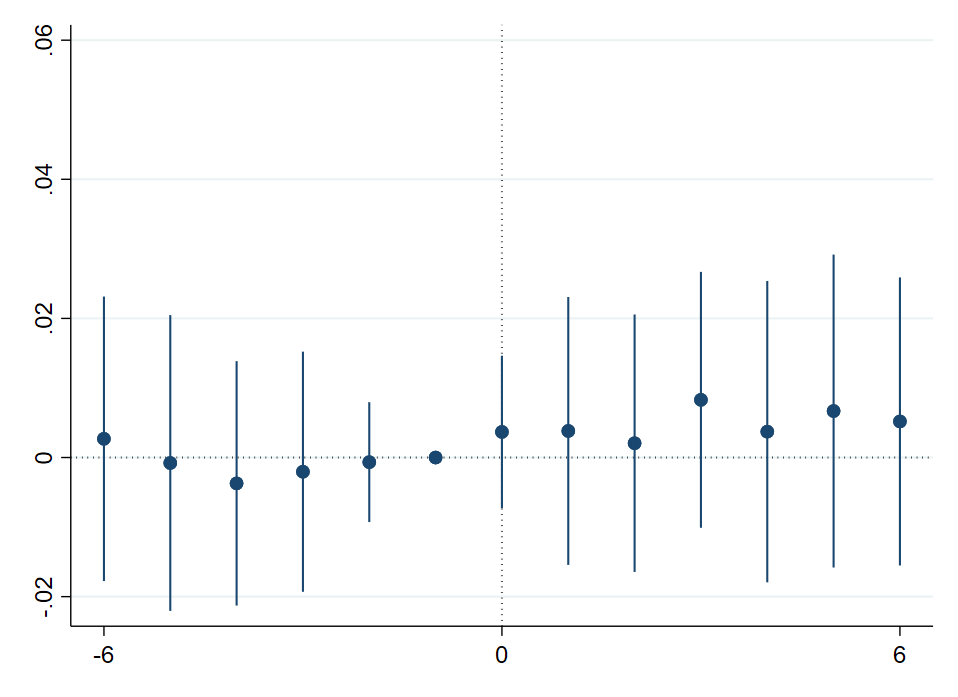
\includegraphics[width=0.95\linewidth]{analysis/event_study_exploration/output/last_rentpsqft_sfcc_cfe_w6.png}
            \caption{Replacing zipcode with county FE} \label{fig:event_study_countyFE_treated}
        \end{subfigure}%
        \begin{subfigure}{0.5\textwidth} \centering
            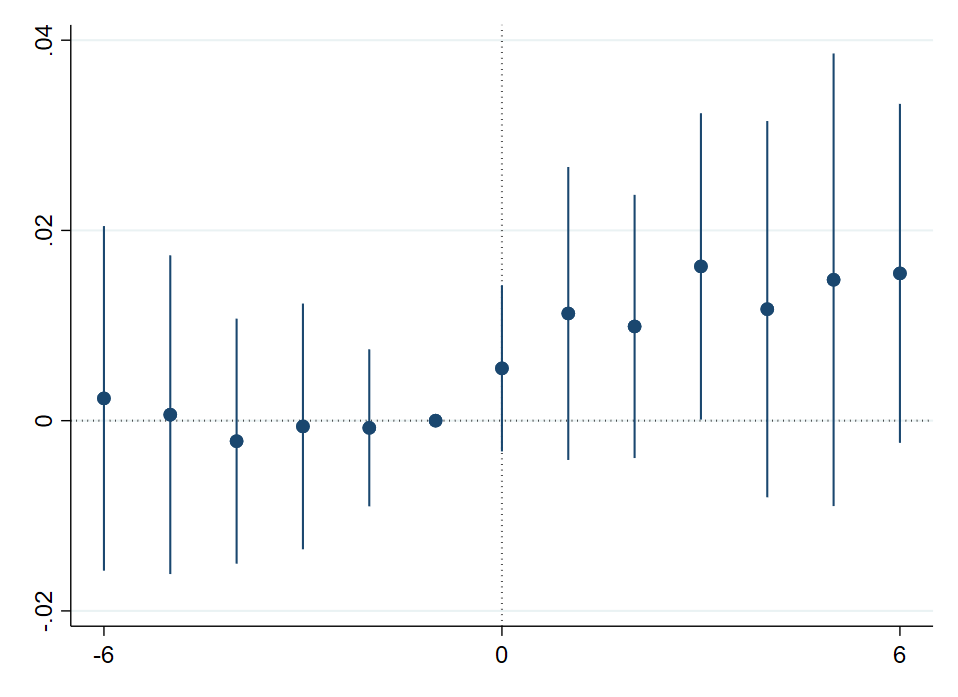
\includegraphics[width=0.95\linewidth]{analysis/event_study_exploration/output/last_rentpsqft_sfcc_cfe_w6_county-trend.png}
            \caption{\begin{tabular}{c} Replacing zipcode with county FE \\ and county-specific trend \end{tabular}} \label{fig:event_study_countyFE_treated_county-trends}
        \end{subfigure}\\
        \begin{subfigure}{0.5\textwidth} \centering
            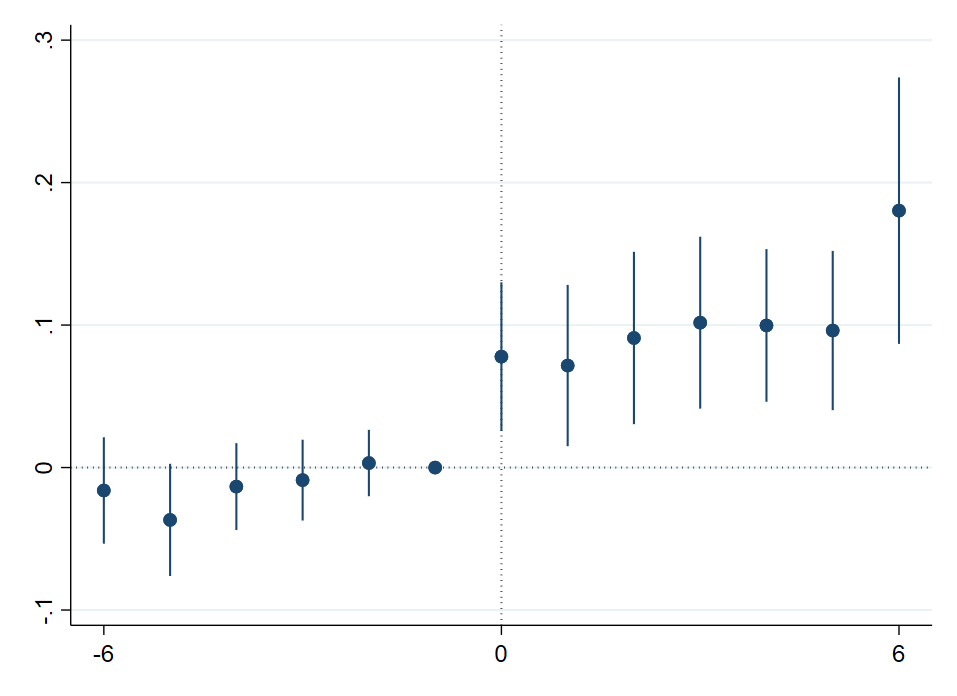
\includegraphics[width=0.95\linewidth]{analysis/event_study/output/last_rentpsqft_sfcc_w6.png}
            \caption{Basic TWFE with untreated units} \label{fig:event_study_all}
        \end{subfigure}%
        \begin{subfigure}{0.5\textwidth} \centering
            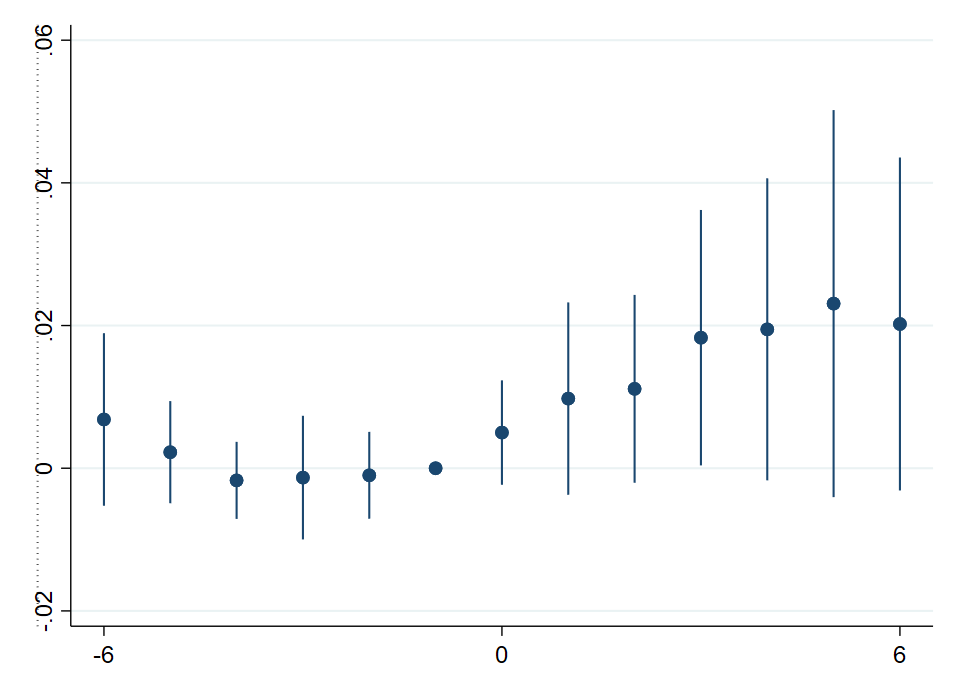
\includegraphics[width=0.95\linewidth]{analysis/event_study/output/last_rentpsqft_sfccw6_county-trend.png} \label{fig:event_study_all_county-trends}
            \caption{\begin{tabular}{c} Basic TWFE with untreated units \\ and county-specific trend \end{tabular}}
        \end{subfigure}\\
        \begin{minipage}{.95\textwidth} \footnotesize
			\vspace{2mm} 
			\textit{Notes}: The figure shows the results from fitting the ``last event'' event study in different samples and with changing controls. In all cases, we select the last minimum wage event per zipcode, based on the requirement that the increase was of at least \$0.5 and that it took place before June 2019 (so that every event has at least 6 months after it). Furthermore, all models: use median rent per square foot of the SFCC category, and control for calendar time fixed effects (FE) and dummies for different categories of the cumulative sum of unused MW events. Each row is a different specification, with the panels on the right adding as controls county-specific linear and quadratic trend. Panels (a) and (b) fit the under-identified model using zipcode FE excluding never treated units (equation \ref{eq:last-event-study}), $N = 46,119$. Panels (c) and (d) use FE at the level of the county instead of zipcode, keeping the sample of never treated units only (equation \ref{eq:last-event-study-countyFE}), $N = 46,119$. Panel (e) and (f) use zipcode FE and add control units (equation \ref{eq:last-event-study-control}), $N = 113,071$.
		\end{minipage}
    \end{figure}
    
    While both panels (c)-(d) and (e)-(f) should solve the under-identification issues raised by \textcite{BorusyakJaravel2017}, we trust more in the results of the bottom panels. The first reason for this is that they maintain zipcode fixed effects, exploiting within zipcode variation in the regression. This seems specially important in light of the conflicting results in \textcite{tidemann2018mw} and \textcite{yamagishi2019minimum}, who use within \textit{county} variation. If only some zipcodes in a county are affected by the change in the minimum wage, then aggregating them up to the county level may mask that effect. 
    
    With the goal of comparing our results to the literature, in Appendix Figure \ref{appfig:event_study_c-q} we aggregate our data to the county quarter level and re-estimate our preferred specification. Panels (a) and (b) estimate the model with a window of 2 quarters, whereas panels (c) and (d) use $w = 4$. All of the estimated coefficients are statistically zero at conventional 95\% confidence levels. Furthermore, the point estimates show inconsistent results. When using a 2-quarter window, they are larger than zero, whereas for a 4-quarter window they seem to be decreasing after the event.\footnote{One partial explanation of this differing behavior is that, since the selection of events depends on the time window, the specifications do not use the same events.} Although more work is required in this vein, we interpret this evidence of suggestive of the importance of using within zipcode variation to estimate the dynamic effects of interest.
    
    The second reason we trust our results of model \eqref{eq:last-event-study-control} in panels (e) and (f) of Figure \ref{fig:event_study_treated} the most more is simply because the sample is 60\% higher than panels (a) to (d), implying that they are more powered to identify an effect. In fact, the confidence intervals seem to be smaller in the bottom row. They increase substantially after the event, which suggests hteregoneity of responses across zipcodes. In the following section we present results of our first difference model, and in that context we explore whether heterogeneous effects are present.
    
    As we discussed in the previous section, the causal claim on these results relies on the assumptions of no pre-trends. Indeed, all estimations show a rather flat and not statistically significant pre-trend. Furthermore, the the pre-event coefficients for panels (e) and (f) are estimated quiet precisely, which implies a strong rejection of the no pre-trends hypothesis. We test for pre-trends formally in our first-differences estimates.
    
    Using this same preferred specification, we explore whether there exists an effect of MW changes on housing prices. We focus on Zillow listings in the same category as we did for rents: single family and condos. We use the variable per square foot to account for potentially changing size of houses in the market. Panel (a) of figure \ref{fig:event_study_main} shows the results without controls for local trends, whereas panel (b) adds county-specific parametric time trends. Whereas the left plot shows what seems to be a null effect (only the estimate on impact is marginally significant), the right plots shows a clear decreasing trend that seems to be not affected by the event. This evidence suggests that the month of the implementation of a minimum wage increase does not impact housing prices. This does not rule out that rents are affected when a new change in the MW is publicly \textit{announced}. Given that housing prices are formed by forward-looking expectations, the relevant event may be different than for rents. We plan to explore this possibility in the future.
    
    \begin{figure}[h!] \centering
        \caption{Dynamic effects around selected minimum wage events: housing prices}
        \label{fig:event_study_main}
        \begin{subfigure}{0.5\textwidth} \centering
            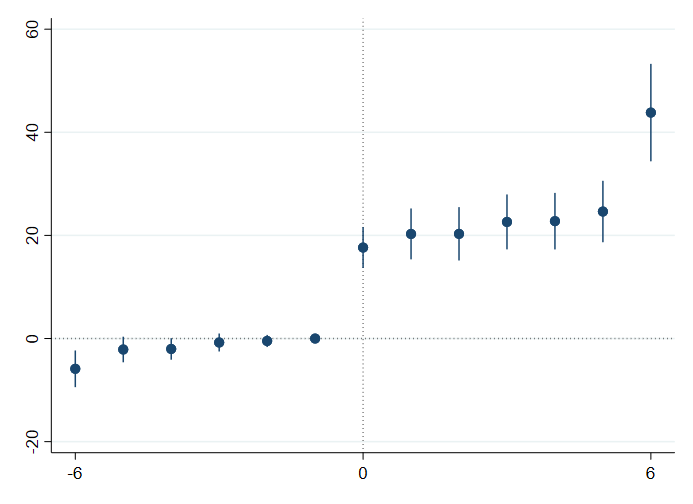
\includegraphics[width=0.95\linewidth]{analysis/event_study/output/last_listingpsqft_sfcc_w6.png}
            \caption{Basic TWFE with all units} \label{fig:event_study_treated}
        \end{subfigure}%
        \begin{subfigure}{0.5\textwidth} \centering
            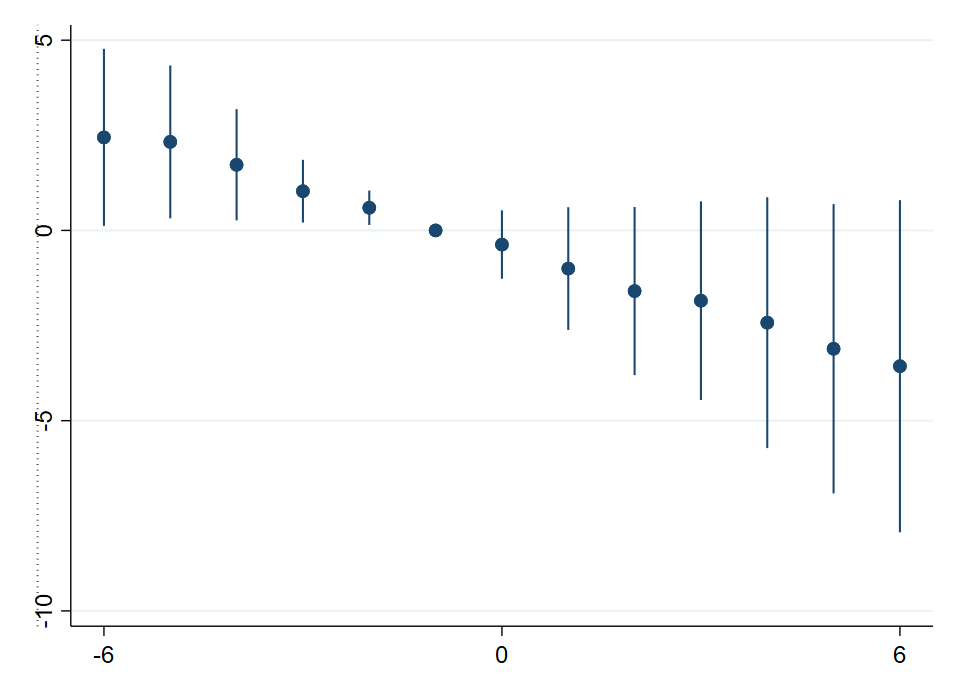
\includegraphics[width=0.95\linewidth]{analysis/event_study/output/last_listingpsqft_sfccw6_county-trend.png}
            \caption{Basic TWFE and county-specific trend} \label{fig:event_study_treated_county-trends}
        \end{subfigure}
        \begin{minipage}{.95\textwidth} \footnotesize
			\vspace{2mm} 
			\textit{Notes}: The figure shows the results from fitting the ``last event'' event study with untreated units on a variable that shows the median housing price per square foot among Zillow postings in the SFCC category within a given zipcode. In all cases, we select the last minimum wage event per zipcode, based on the requirement that the increase was of at least \$0.5 and that it took place before June 2019 (so that every event has at least 6 months after it). Panel (a) fits equation \ref{eq:last-event-study-control}, whereas panel (b) adds county-specific county-trends. In both case, the number of observations is $N = 803,656$.
		\end{minipage}
    \end{figure}
    
    Finally, we explore the robustness of the main results in the bottom panels of Figure \ref{fig:event_study_main} to the cut-off used to select events. Recall that we select the last event within each zipcode of at least \$0.50. Figure \ref{appfig:event_size_sensitivity} explores variation of this cut-off, by selecting changes of at least \$0.25 or \$0.75 instead.
    
    
    % TRY COUNTY-QUARTER SPECIFICATION
    
\subsection{Panel difference-in-differences specifications}\label{subsec:results/first-differences}

    \subsubsection{Baseline results}
    
    In this section we present the results from models based on section 4.2. \autoref{tab:fd_table} shows results from the static model in first differences. Column 1 reports results only including two way fixed effects. Column 2 adds a zipcode-specific linear trend, and column 3 a zipcode specific quadratic trend. 
    
    \begin{table}[h!] \centering
        \caption{Static model}
        \label{tab:fd_table}
        \scalebox{0.85}{
        {
\def\sym#1{\ifmmode^{#1}\else\(^{#1}\)\fi}
\begin{tabular}{l*{3}{c}}
\hline\hline
          &\multicolumn{1}{c}{(1)}&\multicolumn{1}{c}{(2)}&\multicolumn{1}{c}{(3)}\\
          &\multicolumn{1}{c}{D.ln\_med\_rent\_psqft}&\multicolumn{1}{c}{D.ln\_med\_rent\_psqft}&\multicolumn{1}{c}{D.ln\_med\_rent\_psqft}\\
\hline
D.ln\_mw   &   0.0257\sym{*}  &   0.0253\sym{**} &   0.0250\sym{**} \\
          & (0.0128)         & (0.0121)         & (0.0117)         \\
\hline
Zipcode-specifc linear trend&       No         &      Yes         &      Yes         \\
Zipcode-specific linear and square trend&       No         &       No         &      Yes         \\
R-squared &                  &                  &                  \\
Observations&    0.022         &    0.023         &    0.026         \\
N         &   113363         &   113363         &   113363         \\
\hline\hline
\end{tabular}
}
}
        \begin{minipage}{.95\textwidth} \footnotesize
			\vspace{3mm} 
			\textit{Notes}: The table shows the estimated impact of a change in MW on change in (log) median rent per square foot from \autoref{eq:diff_main}. Column 1 shows the results of a two way fixed effect version of the model. Column 2 add a zipcode specific linear trend, while Column 3 controls for a zipcode quadratic trend. Robust standard errors clustered at the state level.  
		\end{minipage}
    \end{table}
    
    
    In all cases the effects is significant, stable and a 10\% change in the MW implies around a 0.25\% increase in the rent per square foot. 
    
    Next, in \autoref{tab:fd_dyn_table} we show results from a model with 5 leads and lags of the logarithm of the MW. Again, Column 1 reports results of a specification with two way fixed effects. Column 2 adds a zipcode-specific linear trend, and column 3 a zipcode specific quadratic trend. 
    
    \begin{table}[h!] \centering
        \caption{Dynamic model}
        \label{tab:fd_dyn_table}
        \scalebox{0.85}{
        {
\def\sym#1{\ifmmode^{#1}\else\(^{#1}\)\fi}
\begin{tabular}{l*{5}{c}}
\hline\hline
          &\multicolumn{1}{c}{(1)}         &\multicolumn{1}{c}{(2)}         &\multicolumn{1}{c}{(3)}         &\multicolumn{1}{c}{(4)}         &\multicolumn{1}{c}{(5)}         \\
\hline
$\Delta \ln \underline{w}_{ic,t-5}$&  -0.0148         &  -0.0144         &  -0.0144         &  -0.0146         &  -0.0144         \\
          & (0.0090)         & (0.0089)         & (0.0089)         & (0.0090)         & (0.0089)         \\
[1em]
$\Delta \ln \underline{w}_{ic,t-4}$&  -0.0024         &  -0.0019         &  -0.0020         &  -0.0022         &  -0.0019         \\
          & (0.0116)         & (0.0116)         & (0.0115)         & (0.0116)         & (0.0115)         \\
[1em]
$\Delta \ln \underline{w}_{ic,t-3}$&   0.0011         &   0.0005         &   0.0007         &   0.0004         &  -0.0002         \\
          & (0.0092)         & (0.0094)         & (0.0092)         & (0.0091)         & (0.0092)         \\
[1em]
$\Delta \ln \underline{w}_{ic,t-2}$&   0.0060         &   0.0063         &   0.0062         &   0.0060         &   0.0064         \\
          & (0.0116)         & (0.0118)         & (0.0116)         & (0.0115)         & (0.0117)         \\
[1em]
$\Delta \ln \underline{w}_{ic,t-1}$&  -0.0002         &  -0.0004         &  -0.0005         &   0.0000         &  -0.0005         \\
          & (0.0123)         & (0.0123)         & (0.0124)         & (0.0122)         & (0.0123)         \\
[1em]
$\Delta \ln \underline{w}_{ic,t}$&   0.0271\sym{**} &   0.0257\sym{**} &   0.0259\sym{**} &   0.0269\sym{**} &   0.0259\sym{**} \\
          & (0.0126)         & (0.0123)         & (0.0124)         & (0.0126)         & (0.0124)         \\
[1em]
$\Delta \ln \underline{w}_{ic,t+1}$&   0.0136\sym{*}  &   0.0146\sym{**} &   0.0142\sym{*}  &   0.0135\sym{*}  &   0.0146\sym{*}  \\
          & (0.0072)         & (0.0072)         & (0.0072)         & (0.0072)         & (0.0072)         \\
[1em]
$\Delta \ln \underline{w}_{ic,t+2}$&  -0.0070         &  -0.0066         &  -0.0064         &  -0.0068         &  -0.0064         \\
          & (0.0133)         & (0.0133)         & (0.0132)         & (0.0133)         & (0.0132)         \\
[1em]
$\Delta \ln \underline{w}_{ic,t+3}$&   0.0036         &   0.0045         &   0.0047         &   0.0031         &   0.0040         \\
          & (0.0081)         & (0.0078)         & (0.0078)         & (0.0079)         & (0.0077)         \\
[1em]
$\Delta \ln \underline{w}_{ic,t+4}$&   0.0108         &   0.0093         &   0.0104         &   0.0107         &   0.0096         \\
          & (0.0069)         & (0.0066)         & (0.0064)         & (0.0069)         & (0.0065)         \\
[1em]
$\Delta \ln \underline{w}_{ic,t+5}$&   0.0086         &   0.0095         &   0.0099         &   0.0088         &   0.0099         \\
          & (0.0069)         & (0.0065)         & (0.0065)         & (0.0067)         & (0.0065)         \\
\hline
\vspace{-2mm}&                  &                  &                  &                  &                  \\
Cumulative effect&    0.057         &0.057\sym{*}         &0.059\sym{*}         &    0.056         &0.058\sym{*}         \\
          &  (0.035)         &  (0.034)         &  (0.034)         &  (0.034)         &  (0.034)         \\
\hline    &                  &                  &                  &                  &                  \\
P-value no pretrends&    0.568         &    0.612         &    0.599         &    0.594         &    0.629         \\
Wage controls&       No         &      Yes         &       No         &       No         &      Yes         \\
Employment controls&       No         &       No         &      Yes         &       No         &      Yes         \\
Establishment-count controls&       No         &       No         &       No         &      Yes         &      Yes         \\
R-squared &    0.022         &    0.022         &    0.022         &    0.022         &    0.022         \\
Observations&  106,446         &  105,463         &  105,463         &  106,160         &  105,463         \\
\hline\hline
\end{tabular}
}
}
        \begin{minipage}{.95\textwidth} \footnotesize
			\vspace{3mm} 
			\textit{Notes}:  The table shows the estimated $\beta_{r}$ coefficients from \autoref{eq:diff_dynamic_reg}. Column 1 shows the results of a two way fixed effect version of the model. Column 2 add a zipcode specific linear trend, while Column 3 controls for a zipcode quadratic trend. Robust standard errors clustered at the state level.  
		\end{minipage}
    \end{table}
    
    We also report the p-value of a test of $\beta_{-5} = \beta_{-4} = ... = \beta_{-1} = 0$. In all 3 cases we comfortably fail to reject that all leads are equal to 0 at the 95\% level. This is evidence that the pre-existing time paths of rent per square foot in zipcodes where the MW changed is not significantly different that the one for zipcodes in which the change didn't happened on that same time period. Given this, we estimate a model in which we assume all the leads are 0, and we include 5 lags of the logarithm of the MW (we call this model the distributed lags model). The coefficients from this estimation, plus the ones from the specification including 5 leads and lags are plotted in Figure XXX along with the path of effects implied by the static and distributed lags model. 
    
    \begin{figure}[h!] \centering
        \caption{Implied effect of different models}
        \label{fig:fd_models}
        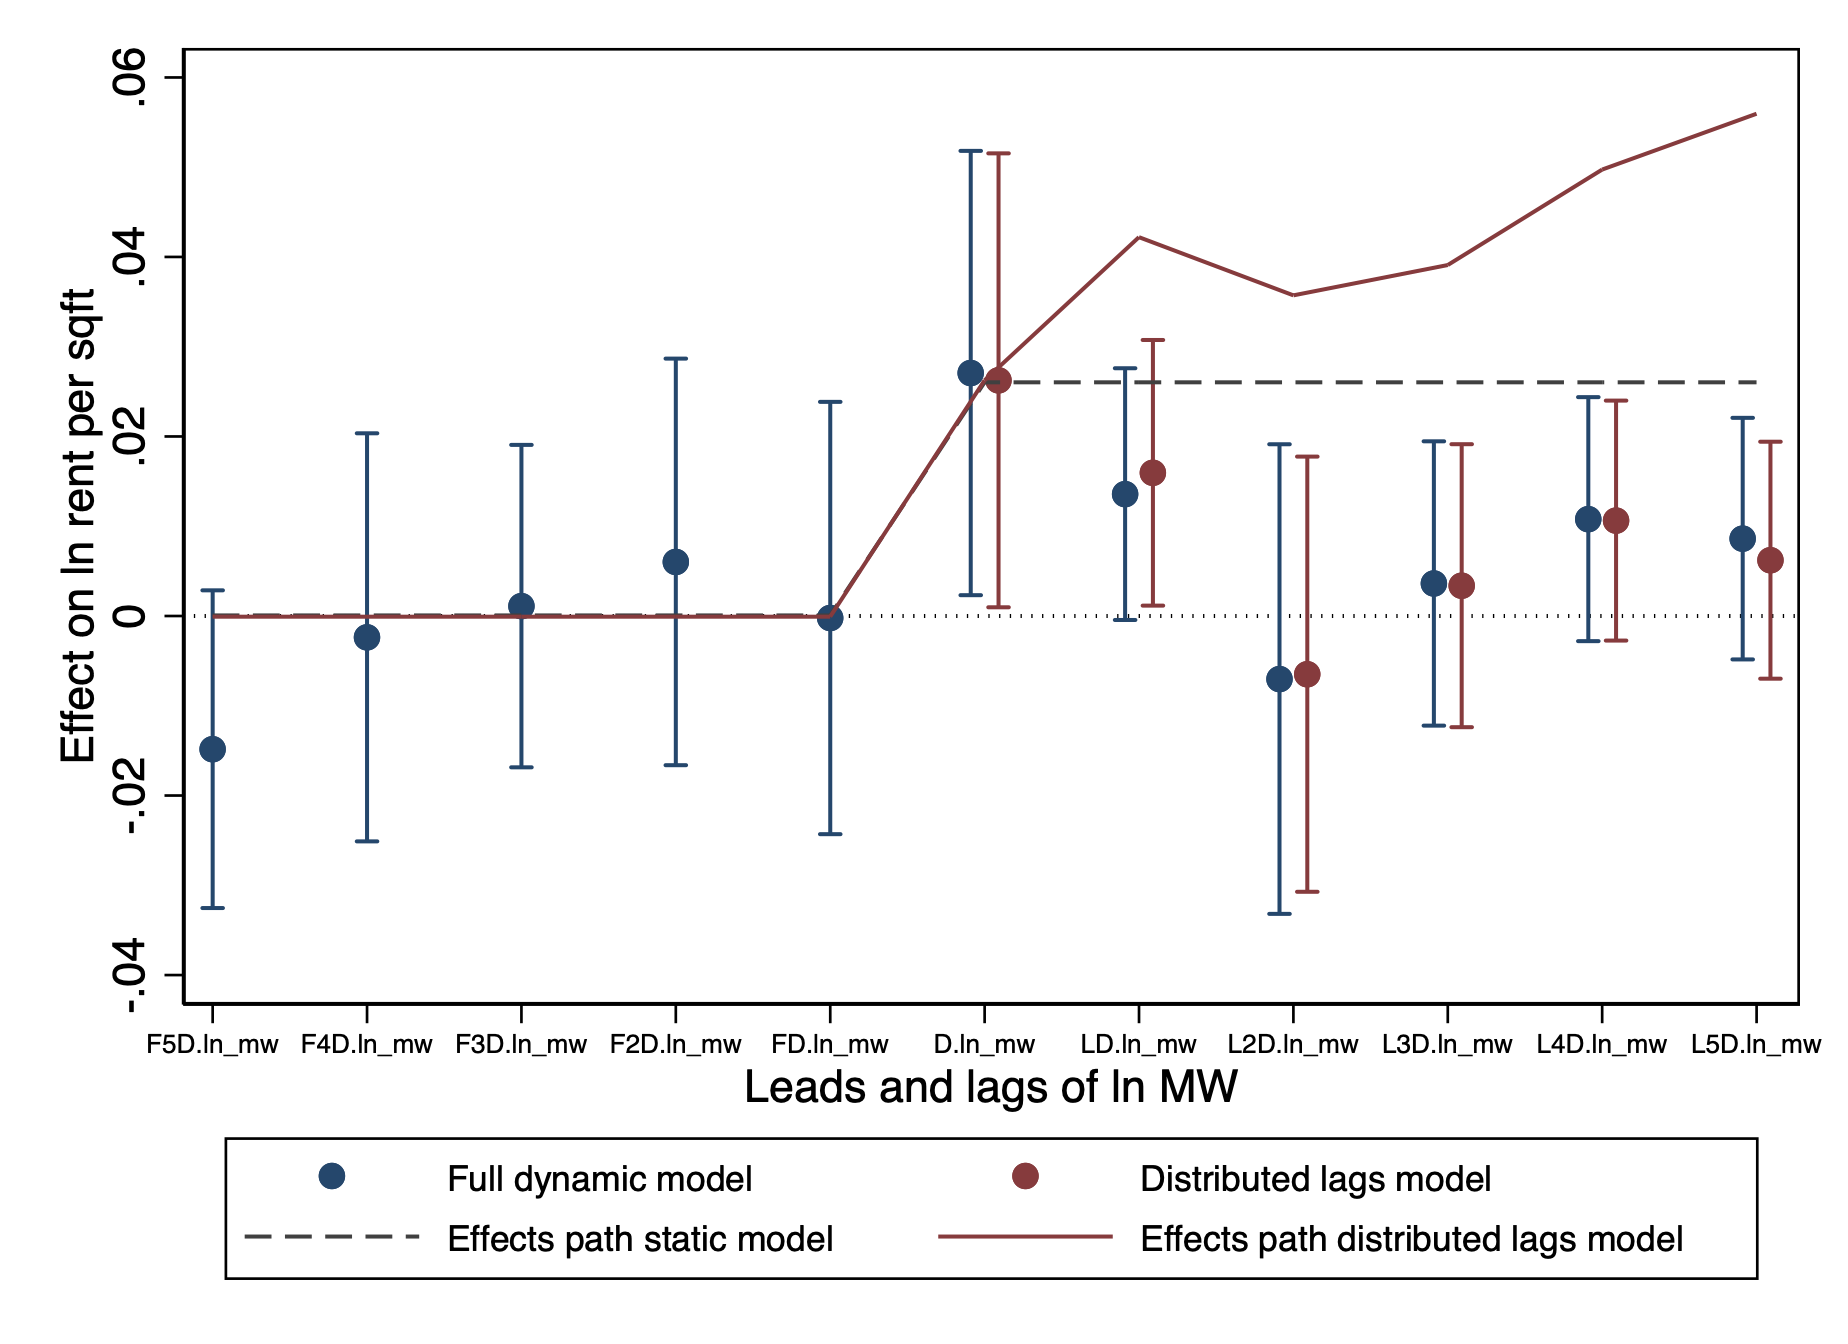
\includegraphics[width=0.75\linewidth]{analysis/first_differences/output/fd_models.png}
        \begin{minipage}{.95\textwidth} \footnotesize
			\vspace{2mm} 
			\textit{Notes}: The figure plots the estimated coefficients from the full dynamic model presented in \autoref{eq:diff_dynamic_reg}; the estimated coefficients from a distributed lag model assuming that all leads are 0; the cumulative effect for such distributed lag model; and the effect estimated through the static model in \autoref{eq:diff_main} (for this last estimate, we omit standard errors estimates for visual clarity). 
		\end{minipage}
    \end{figure}
    
    We can see that there is no evidence of pretrends, and that the effects implied by the dynamic models are slightly larger than the ones implied by the static one.  
    
    
    \subsubsection{Heterogeneity by income}
    
    In order to explore whether the effects of MW on rents are mainly driven by "minimum wager" zipcodes we divide the set of zipcodes into median household income quintiles from the 2010 census and we run the following model:
    
    \begin{equation}\label{eq:diff_main_hetero}
            \Delta \tilde{y}_{it} = \theta_t + \gamma_i + \sum_{q=1}^5 \beta_q \mathds{1}\{i\in q\} \Delta \tilde{MW}_{it}+ \Delta \epsilon_{it}
    \end{equation}
    
    Were $q$ indexes median household income quintiles, and $\mathds{1}\{i\in q\}$ is 1 if zipcode $i$ belongs to the $q$th quintile of median household income. 
    
    The results are displayed in the following figure. As expected, zipcodes in the lower quintile have an effect that significant and much larger in magnitude the baseline effect on the full sample of zipcodes.
    
    Further heterogeneity in Appendix Figure \ref{appfig:fd_heterogeneity_appendix}.
    
    \begin{figure}[h!] \centering
        \caption{Heterogeneity of effect across zipcode median income quintiles}
        \label{fig:fd_heterogeneity_income}
        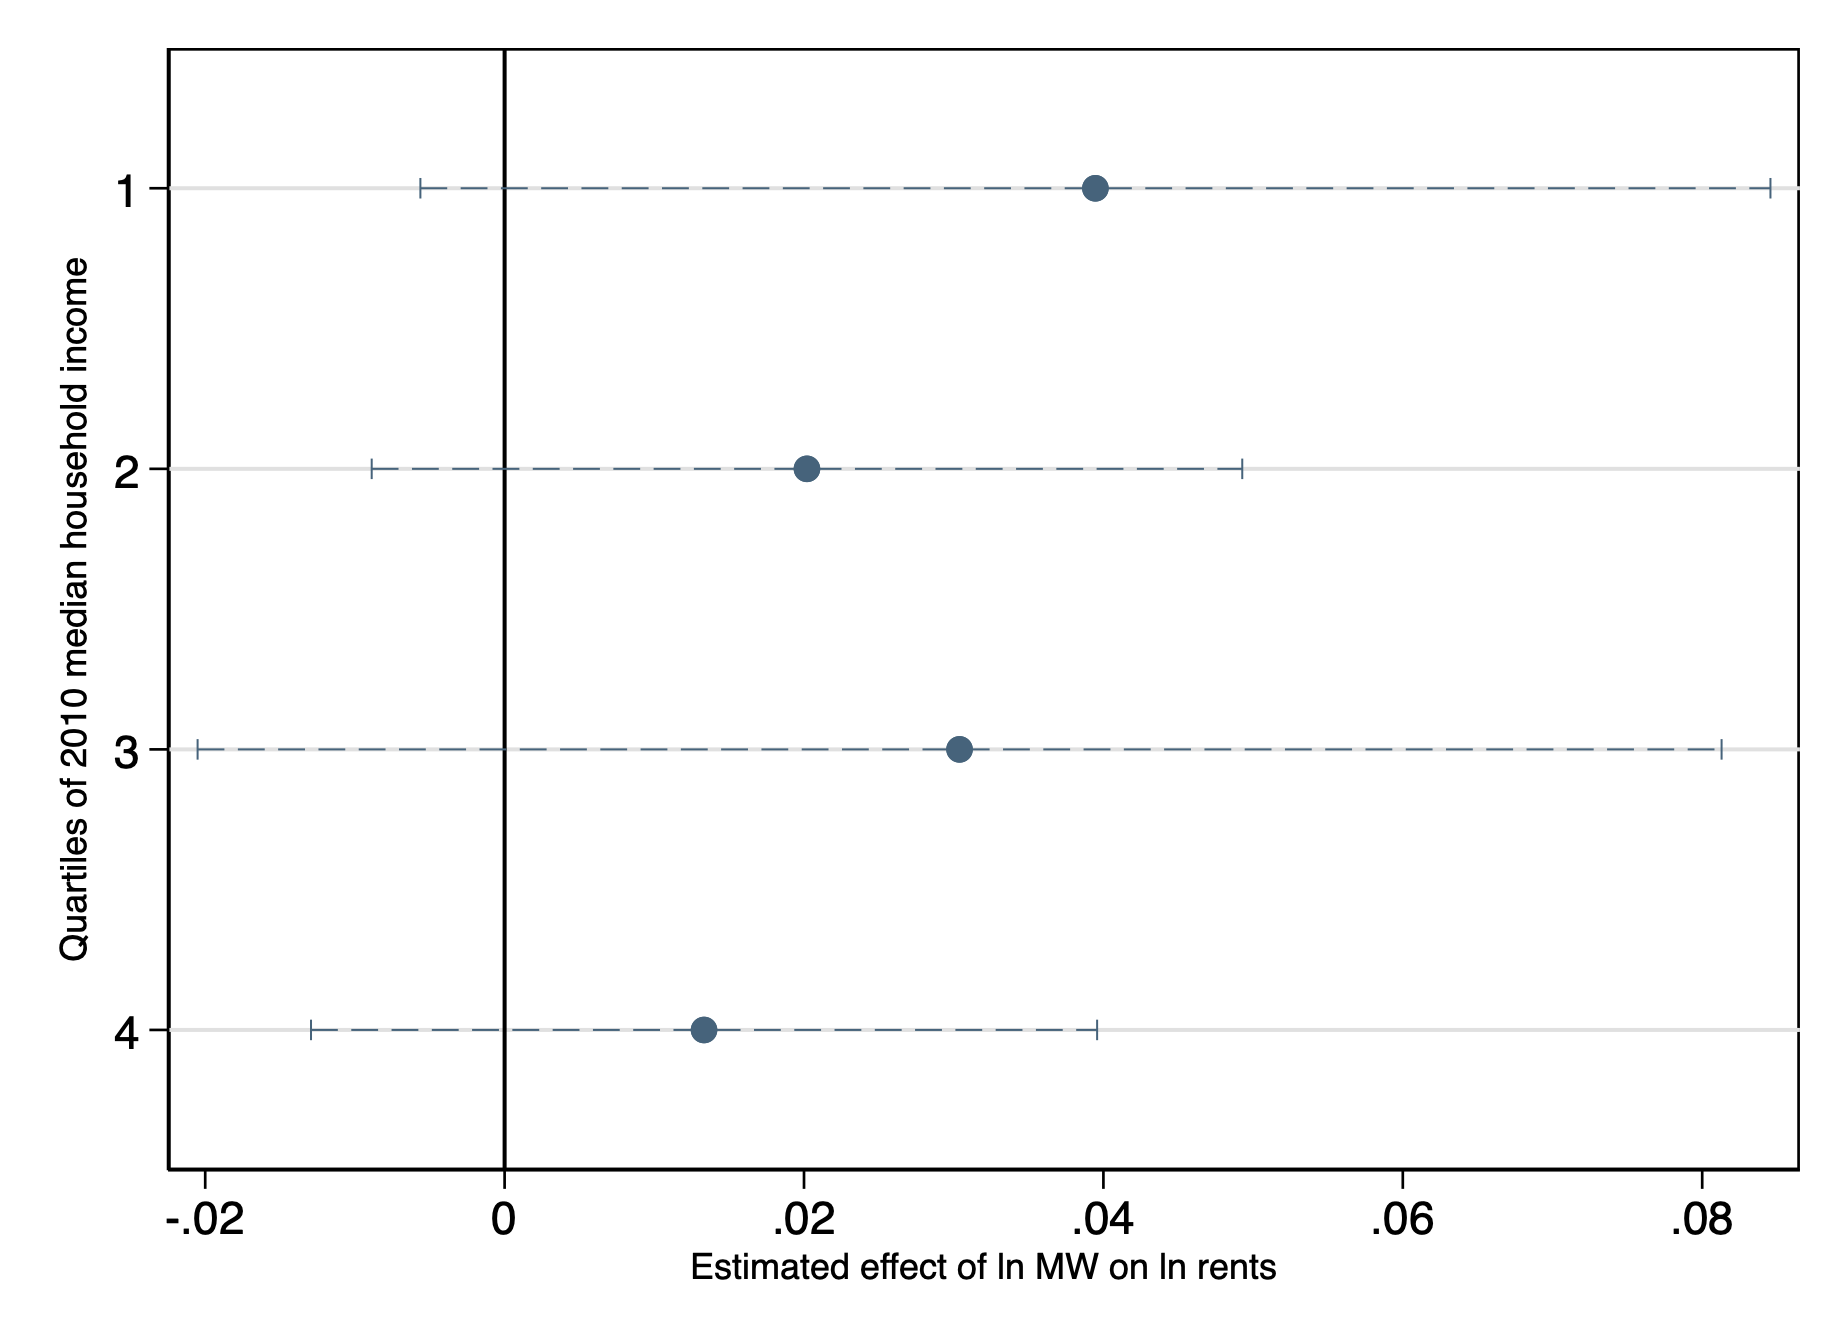
\includegraphics[width=0.75\linewidth]{analysis/first_differences/output/fd_static_heter_med_hhinc20105.png}
        \begin{minipage}{.95\textwidth} \footnotesize
			\vspace{2mm} 
			\textit{Notes}: The plot shows the estimated $\beta_{q}$ coefficients from \autoref{eq:diff_main_hetero}. Robust standard errors clustered at the state level. 
		\end{minipage}
    \end{figure}
    
\subsection{Assessing magnitude of the effects}\label{subsec:results/magnitude}

    [ADD SOMETHING FOR EVENT STUDIES]

    % FROM DIEGO'S PRESENTATION
    In order to get a sense of the magnitudes of our estimated effects we ask ourselves what would happen with the average rent per square foot if the MW were to increase to \$12, as proposed in this policy brief. For simplicity here, we assume that the consumption of house space for rent is fixed at 1000 square feet. We also assume that the binding MW at a hypothetical zipcode before the counterfactual change is the federal level of \$7.25. In our sample the average zipcode pays \$1.2 per rented square foot, while the average zipcode in the lowest income quintile pays around \$1.
    
    A change of the MW from \$7.25 to \$12 is a change of \%65. Based on our estimates from the static model, the change in the rent per square foot in the average zipcode is of 1.7\% raising to around \$1.22. For our hypothetical family that rents 1000 square foot that is an average increase of the total rent price of \$20.4. For the average zipcode in the lowest quintile, our estimates from the static model with heterogeneity imply a change in the rent per square foot of 3.1\% raising to around \$1.03. For our hypothetical household that is an increase in the total rent of \$31.
    
    [COMPARE ACROSS MODELS]
    
    We view our estimates as a lower bound of the true effects for 2 reasons. First, the zipcodes in our sample are richer than the average zipcode in the US, as those are the zipcodes in which Zillow started collecting data earlier in time. Second, our dynamic model implies effects that are larger than the static model, so in that sense our static estimates are probably conservative.
